\documentclass{beamer}
\usepackage{epstopdf}
\usepackage{graphicx}
%\usepackage{amsmath}

\title{Two-Qubit Dynamics with Josephson Qubits}
\author{John Meade \and Dylan Funk}
\date{April 2, 2015}

\begin{document}

\begin{frame}
\titlepage
\end{frame}

%%%%%%%%%%%%%%%%%%%%%%%%%%%%%%%%%%%%%%%%%%%%%%%%%%%%%%%%%%%%
% History
% fairly short?

\begin{frame}
    \vfill
    \centering
    \begin{beamercolorbox}[sep=8pt,center,shadow=true,rounded=true]{title}
        \usebeamerfont{title}
        History
    \end{beamercolorbox}
    \vfill
\end{frame}

%%% 1

\begin{frame}
    \frametitle{History}
    \framesubtitle{Topic of this slide}
\end{frame}

%%% 2

\begin{frame}
    \frametitle{History}
    \framesubtitle{Topic of this slide}
\end{frame}

%%%

\begin{frame}
    \begin{figure}[ht!]
        \centering
        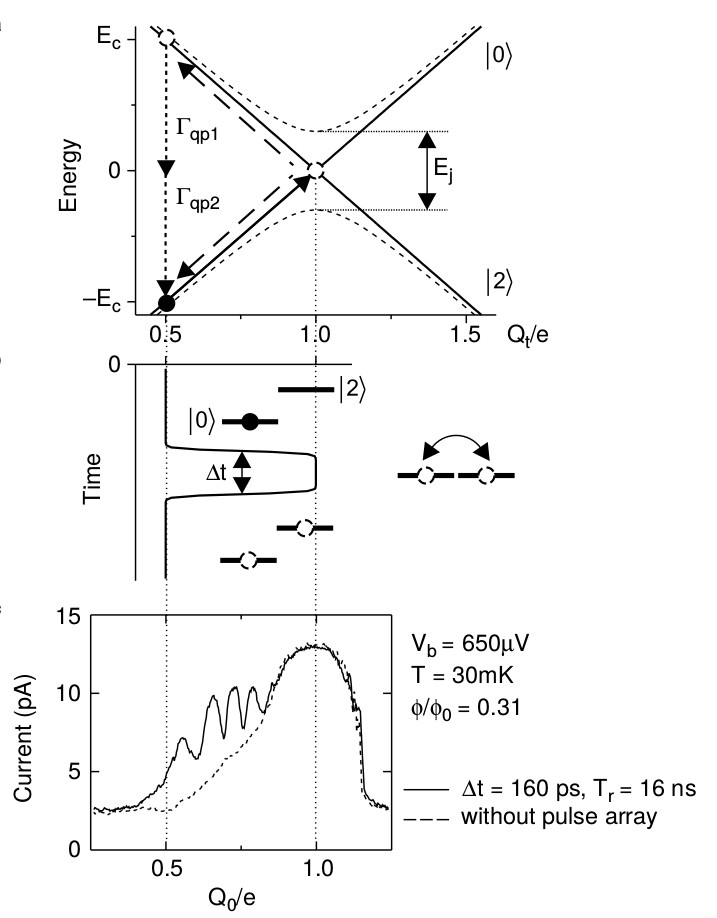
\includegraphics[height=0.8\textheight]{img/single-qubit-band-diagram.jpg}
        \caption{A simple caption}
    \end{figure}
\end{frame}

%%%%%%%%%%%%%%%%%%%%%%%%%%%%%%%%%%%%%%%%%%%%%%%%%%%%%%%%%%%%
% Coupling of Two Qubits
% bulk of presentation here.
% should use 2-column layout often, to compare
% the one-qubit SQUID graphs to the graphs in the paper

\begin{frame}
    \vfill
    \centering
    \begin{beamercolorbox}[sep=8pt,center,shadow=true,rounded=true]{title}
        \usebeamerfont{title}
        Coupling of Two Qubits
    \end{beamercolorbox}
    \vfill
\end{frame}

%%%

\begin{frame}
    \frametitle{Coupling of Two Qubits}
    \framesubtitle{Review}
    \begin{figure}[!htb]
        \centering
        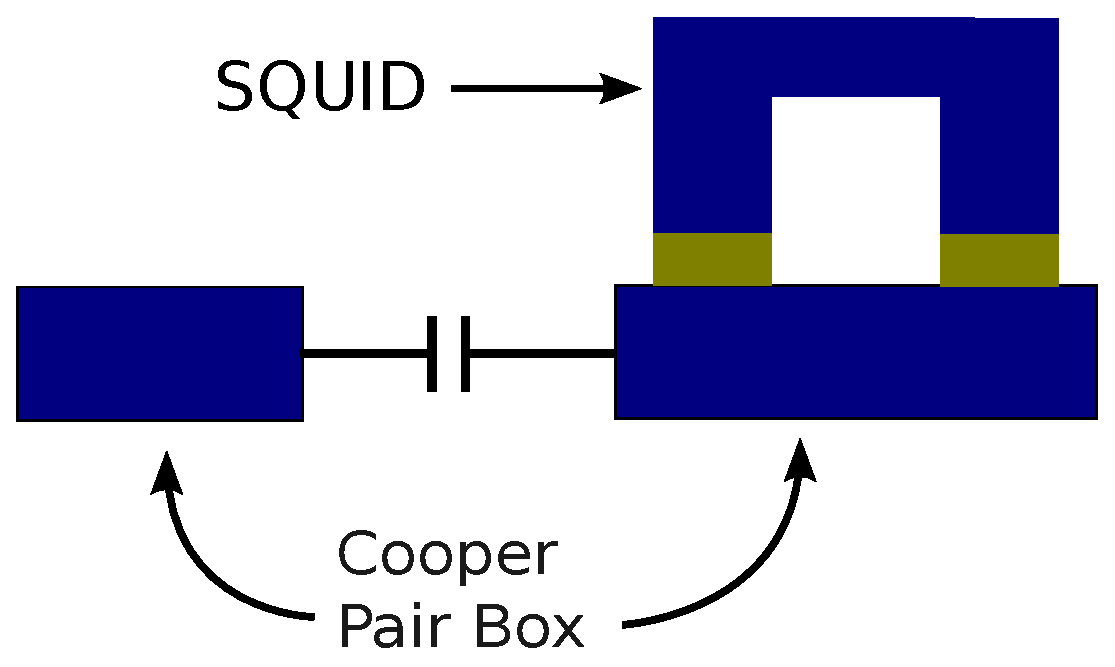
\includegraphics[width=0.8\textwidth]{img/basic-structure.eps}
        %\caption{Digraph.}
        %\label{fig:digraph}
    \end{figure}
\end{frame}

%%%

\begin{frame}
    \frametitle{Coupling of Two Qubits}
    \framesubtitle{Basic Idea}
    \begin{figure}[!htb]
        \centering
        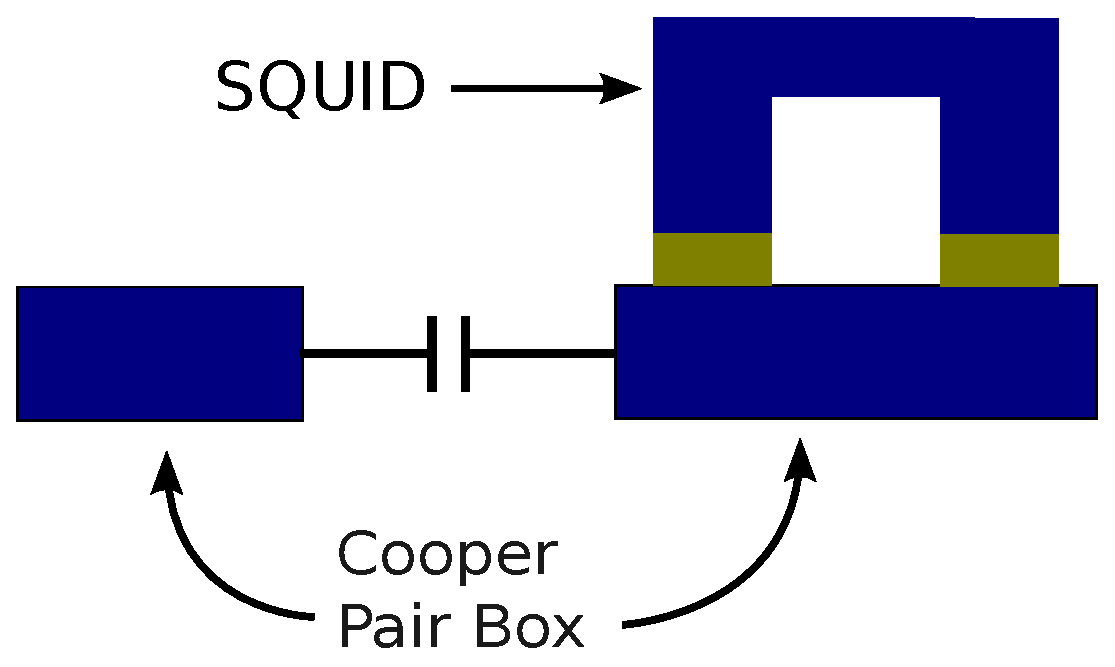
\includegraphics[width=0.8\textwidth]{img/basic-structure.eps}
        %\caption{Digraph.}
        %\label{fig:digraph}
    \end{figure}
\end{frame}

%%%

\begin{frame}
    \frametitle{Coupling of Two Qubits}
    \framesubtitle{Parameter Measurements}
\end{frame}

%%%

\begin{frame}
    \frametitle{Coupling of Two Qubits}
    \framesubtitle{Charging Diagram of Single-Qubit Case}
        \begin{figure}[ht!]
            \centering
            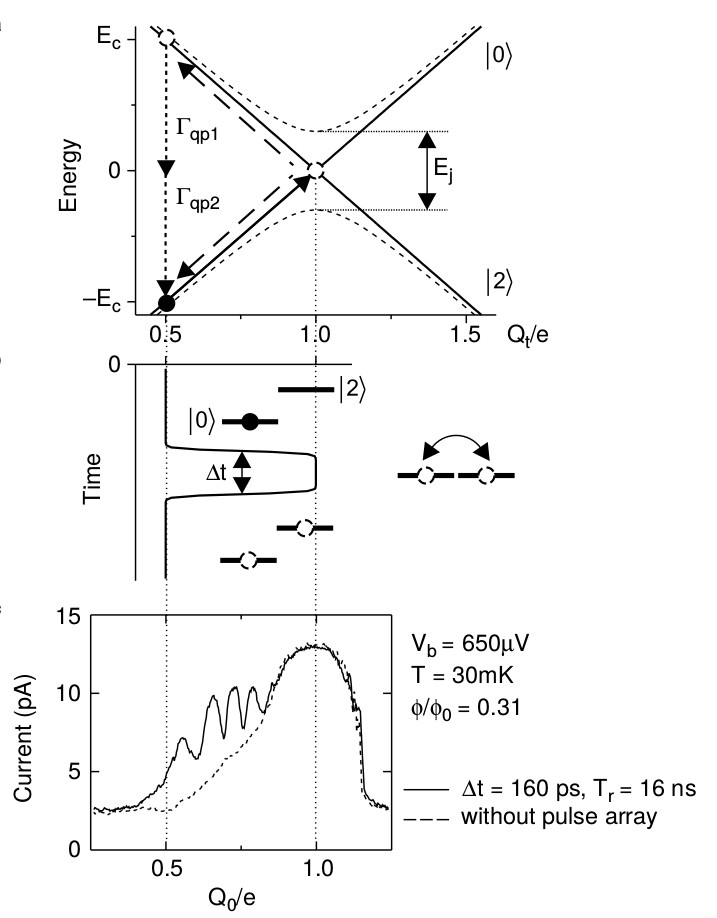
\includegraphics[height=0.6\textheight]{img/single-qubit-band-diagram.jpg}
            \caption{http://www.nature.com/nature/journal/v398/n6730/abs/398786a0.html}
        \end{figure}
\end{frame}

%%%

\begin{frame}
    \frametitle{Coupling of Two Qubits}
    \framesubtitle{Charging Diagram of Two-Qubit Case}
        \begin{figure}[ht!]
            \centering
            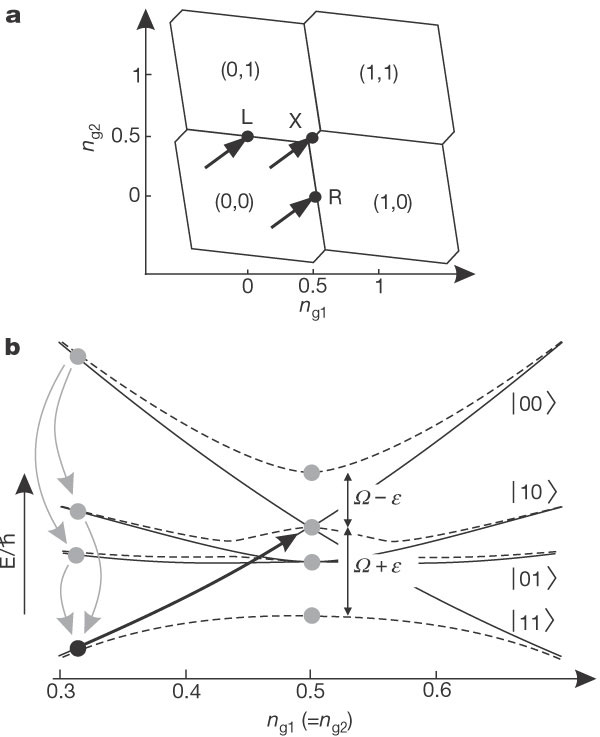
\includegraphics[height=0.6\textheight]{img/charging-diagram.jpg}
            \caption{http://www.nature.com/nature/journal/v421/n6925/full/nature01365.html}
        \end{figure}
\end{frame}

%%%

\begin{frame}
    \frametitle{Coupling of Two Qubits}
    \framesubtitle{State Readout}
    \begin{figure}[!htb]
        \centering
        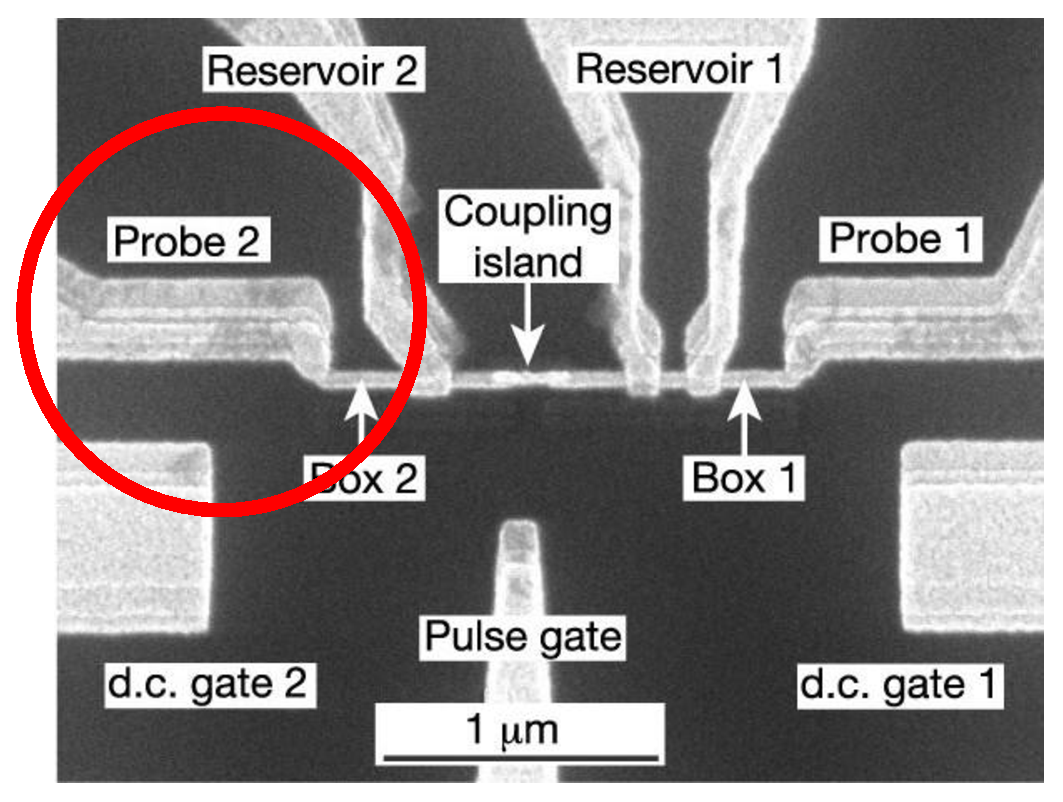
\includegraphics[width=0.8\textwidth]{img/two-qubit-sem-probe.eps}
        %\caption{Digraph.}
        %\label{fig:digraph}
    \end{figure}
\end{frame}

%%%%%%%%%%%%%%%%%%%%%%%%%%%%%%%%%%%%%%%%%%%%%%%%%%%%%%%%%%%%
% Fabrication Techniques

\begin{frame}
    \vfill
    \centering
    \begin{beamercolorbox}[sep=8pt,center,shadow=true,rounded=true]{title}
        \usebeamerfont{title}
        Fabrication Techniques
    \end{beamercolorbox}
    \vfill
\end{frame}

%%% 1

\begin{frame}
    \frametitle{Fabrication Techniques}
    \framesubtitle{Evapouration (Deposition)}
    \begin{figure}[!htb]
        \centering
        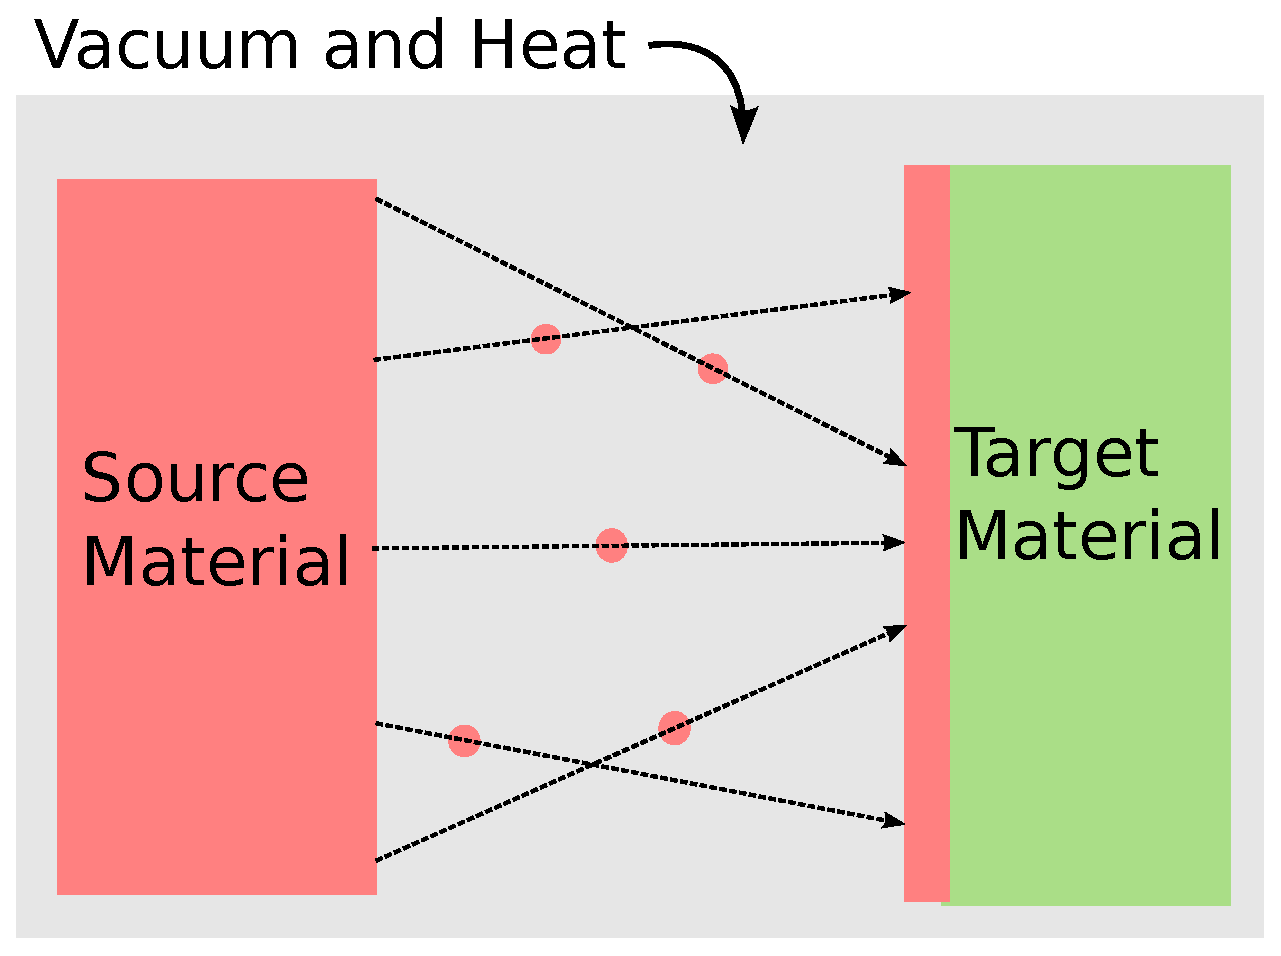
\includegraphics[width=0.8\textwidth]{img/evaporation.eps}
        %\caption{Digraph.}
        %\label{fig:digraph}
    \end{figure}
\end{frame}

%%% 2

\begin{frame}
    \frametitle{Fabrication Techniques}
    \framesubtitle{Electron Beam Lithography (EBL)}
    \begin{figure}[!htb]
        \centering
        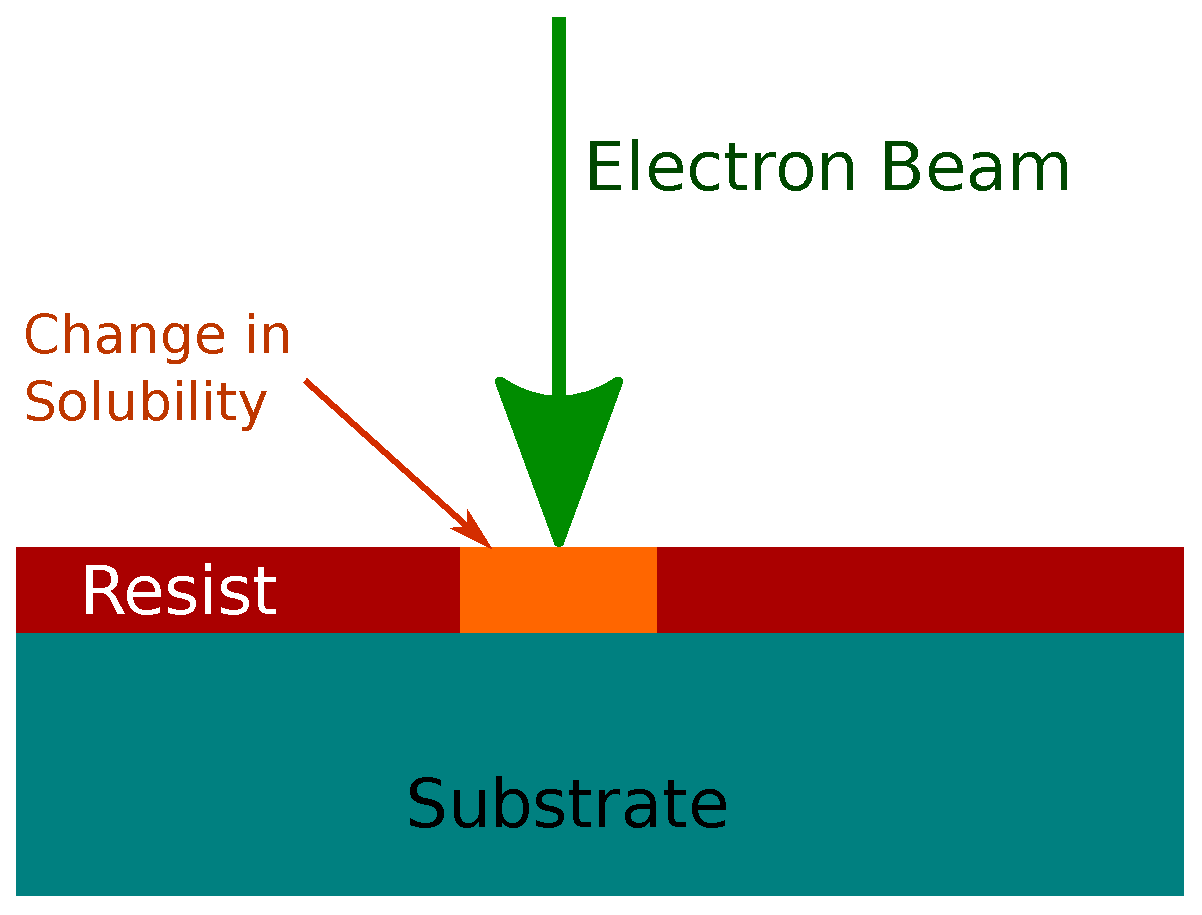
\includegraphics[height=0.8\textheight]{img/ebeam.eps}
    \end{figure}
\end{frame}

%%% 3

\begin{frame}
    \frametitle{Fabrication Techniques}
    \framesubtitle{Etching}
    \begin{figure}[ht!]
        \centering
        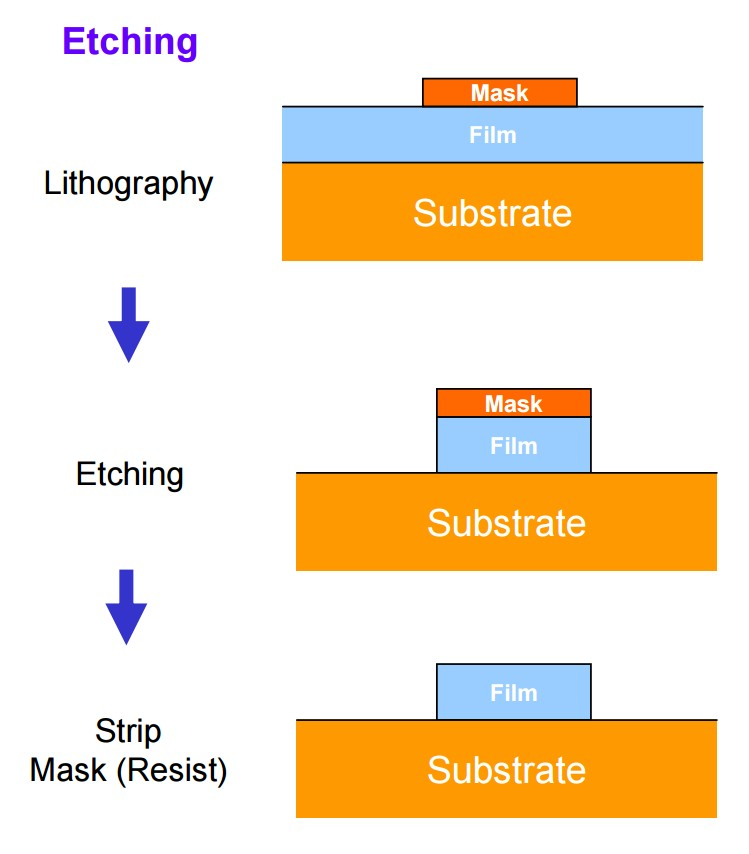
\includegraphics[height=0.6\textheight]{img/etching.jpg}
        \caption{http://www.mrsec.harvard.edu/education/ap298r2004/Erli\%20chen\%20Fabrication\%20III\%20-\%20Etching.pdf}
    \end{figure}
\end{frame}

%%% 4

\begin{frame}
    \frametitle{Fabrication Techniques}
    \framesubtitle{Lift-off}
    \begin{figure}[!htb]
        \centering
        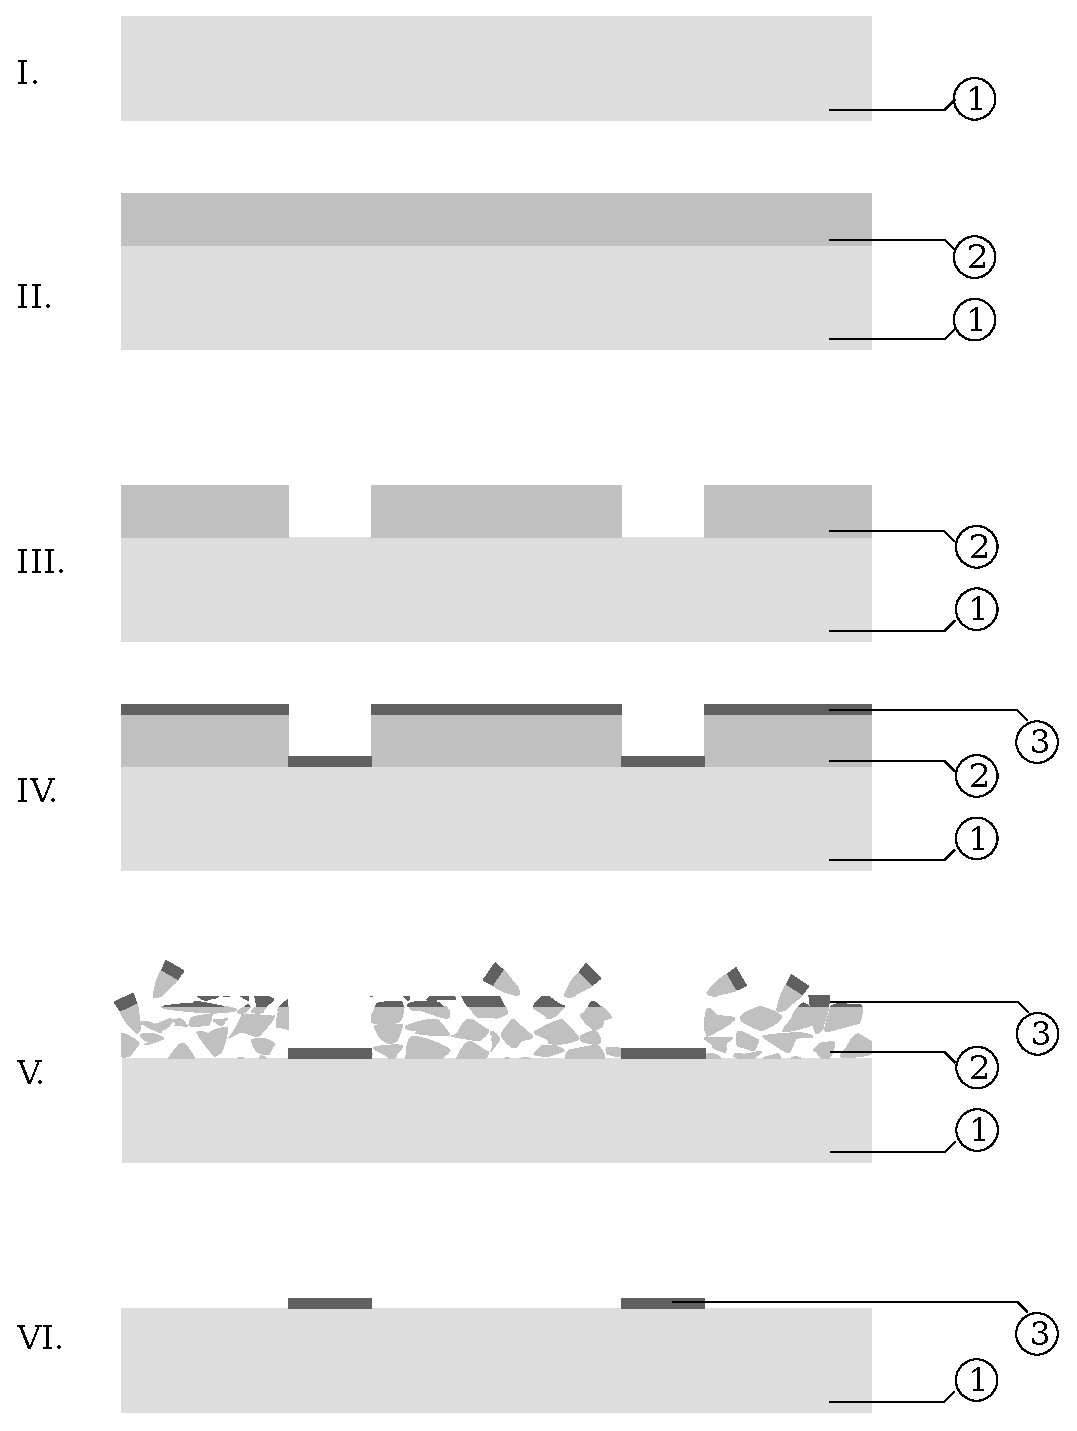
\includegraphics[height=0.6\textheight]{img/lift-off.eps}
        \caption{http://en.wikipedia.org/wiki/Lift-off\_\%28microtechnology\%29}
        %\label{fig:digraph}
    \end{figure}
\end{frame}

%%% 5

\begin{frame}
    \frametitle{Fabrication Techniques}
    \framesubtitle{SEM image of a SQUID qubit}
    \begin{figure}[ht!]
        \centering
        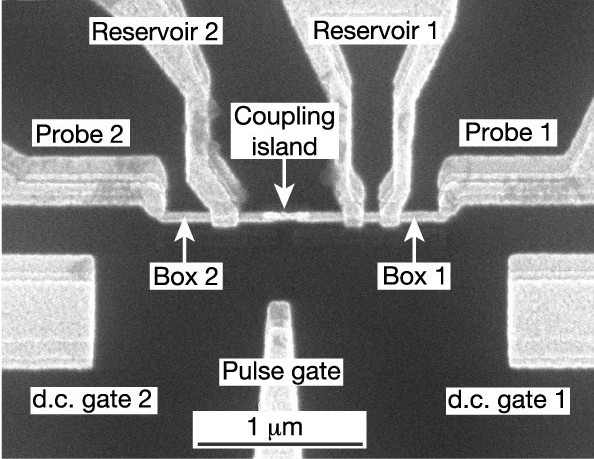
\includegraphics[width=0.7\textwidth]{img/two-qubit-sem.jpg}
        \caption{http://www.nature.com/nature/journal/v421/n6925/full/nature01365.html}
    \end{figure}
\end{frame}

%%%%%%%%%%%%%%%%%%%%%%%%%%%%%%%%%%%%%%%%%%%%%%%%%%%%%%%%%%%%

\begin{frame}
    \frametitle{THE END}
    \framesubtitle{THE END}
    \begin{columns}
        \column{.5\textwidth}
            \begin{block}{THE END}
                THE END
            \end{block}
        \column{.5\textwidth}
            \begin{block}{THE END}
                \begin{itemize}
                    \item THE END
                    \item THE END
                    \item THE END
                    \item THE END.
                \end{itemize}
            \end{block}
    \end{columns}
\end{frame}

\end{document}
